
%\section{Pointer-Chasing Data Structures}
\section{Low-Contention Data Structures}
\label{section:pointer_chasing}

In this section we consider data structures with low contention. 
Pointer chasing data structures, 
such as linked-lists and skip-lists, fall in this category.  
These are data structures whose operations  
need to de-reference a non-constant sequence of pointers before completing. 
We assume these data structures support operations 
such as add($x$), delete($x$) and contains($x$), which follow ``next node'' pointers until 
reaching the position of node $x$.
When these data structures are too large to fit in the CPU caches 
and access uniformly random keys,
they incur expensive memory accesses, which cannot be easily predicted, 
making the \emph{pointer chasing} operations the dominating overhead of these data structures.
Naturally, these data structures have provided early examples of the benefits of near-memory 
computing~\cite{hsieh2016accelerating, Hashemi:2016}, 
as the entire pointer chasing operation could be performed by a PIM core with fast memory access, 
and only the final result returned to the application. 

However, these data structures have inherently low contention. 
Lock-free algorithms
~\cite{practicallf, skiplists-concpugh, valois, Herlihy08}
have shown that these data structures can scale to hundreds of cores under low contention~\cite{nodereplication}.
Unfortunately, each vault in 
PIM memory has a single core. 
As a consequence, prior work has only compared PIM data structures with sequential data structures, 
\emph{not} with carefully crafted concurrent data structures.

We analyze linked-lists and skip-lists, and show that the naive PIM data structure in each case cannot 
outperform the equivalent CPU-managed concurrent data structure even for a small number of cores. 
Next, we show how to use state-of-the art techniques from concurrent computing to 
optimize data structures for near-memory computing such that they outperform well-known concurrent data 
structures designed for multi-core CPUs. 

%\subsection{PIM-managed linked-list}
\subsection{Linked-lists}
\label{section:linked_list}
We first describe a naive PIM linked-list.
The linked-list is stored in a vault, maintained by the local PIM core.
Whenever a CPU\footnote{We use the term CPU to refer to a CPU core, as opposed to a PIM core.} 
wants to perform an operation on the linked-list,
it sends a request to the PIM core.
The PIM core then retrieves the message, executes the operation, and sends the result back to the CPU.
The PIM linked-list is sequential, as it can only be accessed by one PIM core. 

Performing pointer chasing on sequential data structures using PIM cores is not a new idea. 
Prior work (\cite{hsieh2016accelerating, Ahn2015:2, Hashemi:2016}) has shown that 
pointer chasing can be done more efficiently by a PIM core for a sequential data structure.
However, we are not aware of any prior comparison between the performance of
PIM-managed data structures and \emph{concurrent} data structures, 
for which CPUs can make operations in parallel.
In fact, our analytical and experimental results show that 
the naive PIM-managed linked-list is not competitive with 
a concurrent linked-list that uses fine-grained locks~\cite{Heller05}.

We use the \textit{combining optimization} proposed by 
flat combining~\cite{Hendler10} to improve this data structure:
a PIM core can execute all concurrent requests by CPU cores using \emph{a single} 
traversal over the linked-list. 

The role of the PIM core in our PIM-managed linked-list
is very similar to that of the combiner in a concurrent linked-list implemented
using \textit{flat combining} \cite{Hendler10}, where, roughly speaking,
threads compete for a ``combiner lock" to become the combiner, and
the combiner takes over all operation requests from other threads and executes them.
Therefore, we consider the performance of the flat-combining linked-list as an indicator 
of the performance of our proposed PIM-managed linked-list.

Based on our performance model, we can calculate the approximate expected throughput 
(in operations per second) of each of the linked-lists mentioned above, 
when there are $p$ CPUs making operation requests concurrently.
We assume that a linked-list consists of nodes with integer keys in the range of $[1, N]$.
Initially a linked-list has $n$ nodes with keys generated independently
and uniformly at random from $[1, N]$.
The keys of the operation requests are generated the same way.
To simplify the analysis, we assume that the size of the linked-list does not fluctuate much. 
This is achieved when the number of add() requests is similar to the number of delete() requests. 
We assume that a CPU makes a new operation request immediately after
its previous one completes.
Assuming that $n \gg p$ and $N \gg p$, the approximate expected throughput (per second) of each
of the concurrent linked-lists is presented in Table \ref{tab:linkedlist}, 
where $\Sp = \sum\limits_{i=1}^{n} ({i \over n+1})^{p}$.

\renewcommand{\arraystretch}{1.6}
\begin{table}[ht!]
\begin{center}
    \begin{tabular}{| >{\small}l | l |}
	%\begin{tabular}{| m{0.68\linewidth}  | c |}    
    \hline
    \textbf{Algorithm} & \textbf{Throughput}\\ \hhline{|=|=|}
    Linked-list with fine-grained locks & ${2p \over (n+1)\latcpu}$ \\ \hline
    Flat-combining linked-list without combining & ${2 \over (n+1)\latcpu}$ \\ \hline
    PIM-managed linked-list without combining & ${2 \over (n+1)\latpim}$ \\ \hline
    Flat-combining linked-list with combining & ${p \over (n-\Sp)\latcpu}$ \\ \hline
    PIM-managed linked-list with combining & ${p \over (n-\Sp)\latpim}$ \\ \hline
    \end{tabular}
\end{center}
\caption{Throughput of linked-lists}
\label{tab:linkedlist}
\end{table}

We calculate the throughput values in Table \ref{tab:linkedlist} in the following manner. 
In the linked-list with fine-grained locks, which has $(n+1)$ nodes including 
a dummy head node, each thread (CPU) executes its own operations to the linked-list. 
The key of a request is generated uniformly at random, 
so the average number of memory accesses by one thread for one operation is $(n+1)/2$ 
and hence the throughput of one thread is $2/((n+1)\latcpu)$. 
There are $p$ threads running in parallel, so the total throughput is $2p/((n+1)\latcpu)$. 
The throughput of the flat-combining and the PIM-managed linked-lists without the combining optimization 
is calculated in a similar manner. 
For the flat-combining and the PIM-managed linked-lists with combining, it suffices to prove that
the average number of memory accesses by a PIM core (or a combiner) batching and executing 
$p$ random operation requests in one traversal is $n - \Sp$, 
which is essentially the expected number of pointers a PIM core (or a combiner) 
needs to go through to reach the position for the request with the largest key among the $p$ requests. 
Note that we have ignored certain communication costs incurred in some linked-lists, 
such as the latency of a PIM core sending a result back to a waiting thread, 
and the latency of a combiner maintaining the combiner lock and the publication list in the flat-combining 
linked-list (we will discuss the publication list in more detail in Section \ref{section:contended}), 
as they are negligible compared to the dominant costs of traversals over linked-lists.
 
It is easy to see that the PIM-managed linked-list with combining outperforms 
the linked-list with fine-grained locks, which is the best one among other linked-lists, 
if ${\latcpu \over \latpim} = r_1 > {2(n - \Sp)\over n + 1}$.
Given that $0 < \Sp \le {n \over 2}$, 
the PIM-managed linked-list can outperform the linked-list with fine-grained locks as long as $r_1 \ge 2$. 
If we assume $r_1 = 3$, as estimated by prior work, the throughput of the PIM-managed linked-list with 
combining should be at least 1.5 times the throughput of the linked-list with fine-grained locks.
Without combining, however, the PIM-managed linked-list \emph{cannot}
outperform the linked-list with fine-grained locks accessed by $p \ge r_1$ concurrent threads.
On the other hand, the PIM-managed linked-list is expected to be $r_1$ times better than 
the flat-combining linked-list, with or without the combining optimization applied to both.  

We implemented the linked-list with fine-grained locks and the flat-combining linked-list 
with and without the combining optimization.
We tested them on a Dell server with 512 GB RAM and 
56 cores on four Intel Xeon E7-4850v3 processors running at 2.2 GHz.
To eliminate NUMA access effects, we ran experiments with only one processor, 
which is a NUMA node with 14 cores, a 35 MB shared L3 cache, 
and a private L2/L1 cache of size 256 KB/64 KB per core. 
Each core has 2 hyperthreads, for a total of 28 hyperthreads. 

The throughput of each of the linked-lists, measured in operations per second,
is presented in Figure \ref{figure:linkedlist_data}. 
The results confirm the validity of our analysis in Table \ref{tab:linkedlist}.
The throughput of the flat-combining linked-list without the combining optimization
is worse than the linked-list with fine-grained locks.
Since the throughput of the flat-combining linked-list is a good 
indicator of the performance of the PIM-managed linked-list, 
we triple the throughput of the flat-combining linked-list to obtain the expected throughput 
of the PIM-managed linked-list, based on the assumption that $r_1 = 3$. 
As we can see, it is still below the throughput of the one with fined-grained locks.
However, with the combining optimization, the performance of the flat-combining
linked-list improves significantly and our PIM-managed
linked-list with the combining optimization now outperforms all other data structures. 
We conclude that our PIM-managed linked-list is effective.

\begin{comment}
\begin{figure}[ht!]
    \centering
    \begin{minipage}{0.45\linewidth}
        \centering
        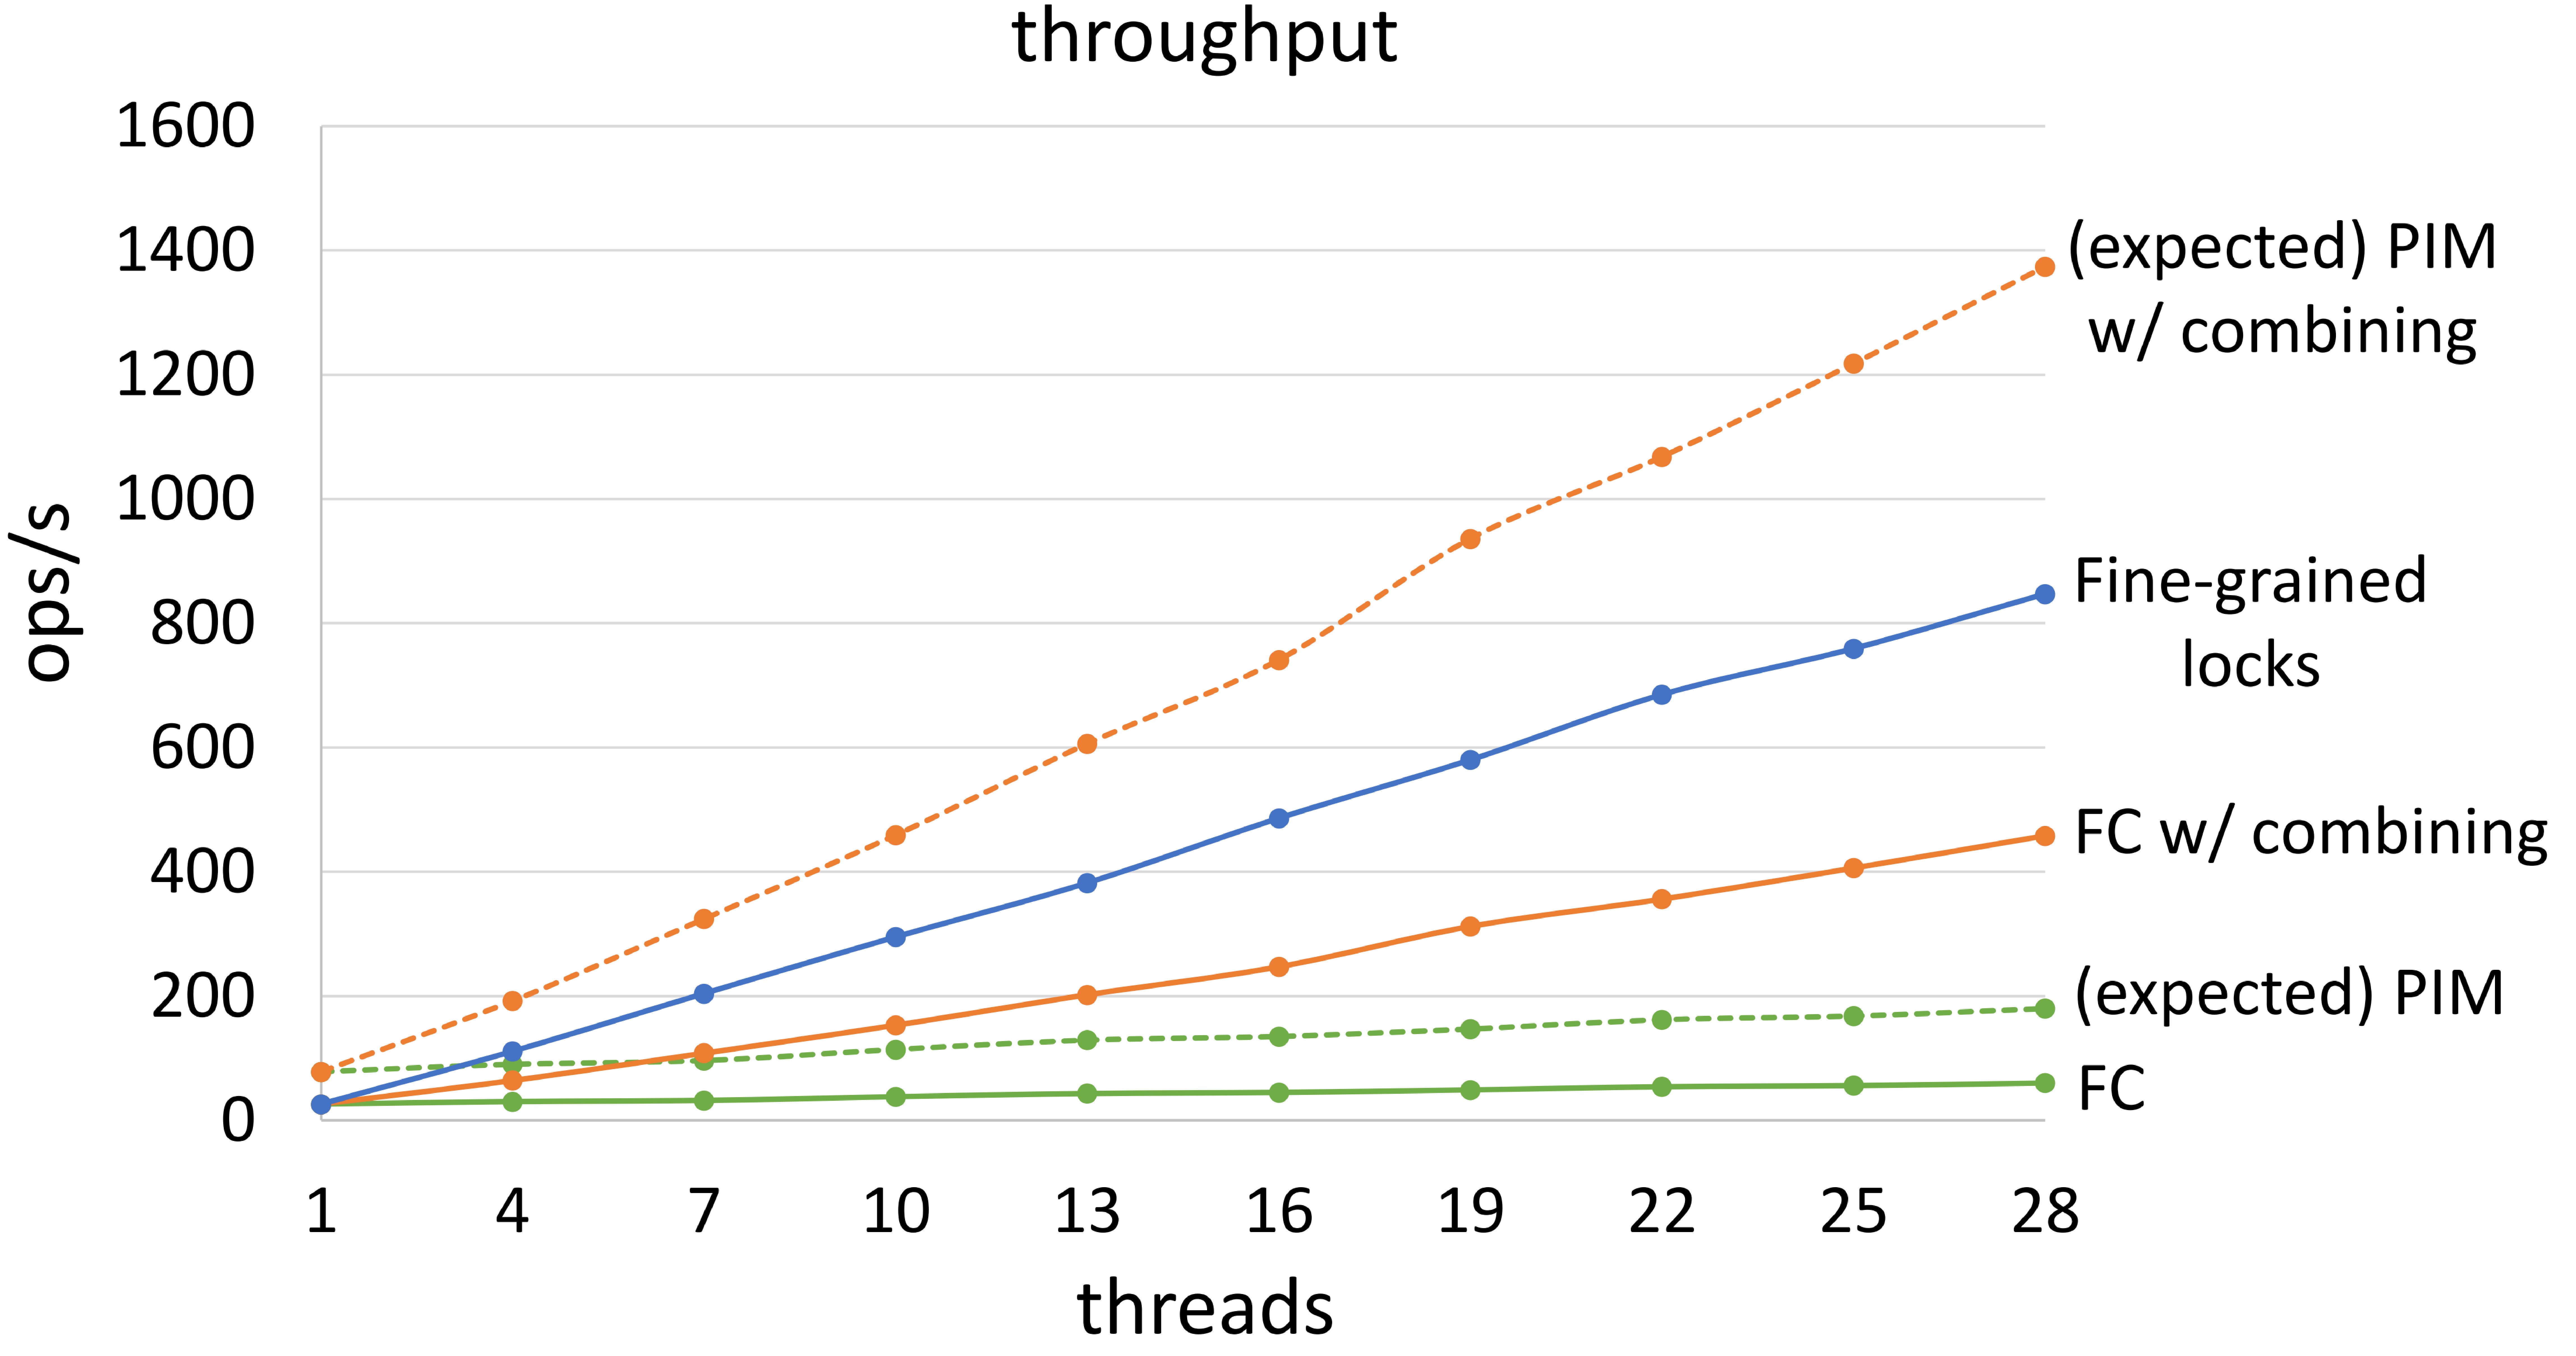
\includegraphics[width=.9\linewidth]{linkedlist_data.eps} % first figure itself
        \caption{Experimental results of linked-lists}
        \label{figure:linkedlist_data}
    \end{minipage}\hfill
    \begin{minipage}{0.45\linewidth}
        \centering
        
\includegraphics[width=.98\linewidth]{skiplist_data.eps} % second figure itself
        \caption{Experimental results of skip-lists}
        \label{figure:skiplist_data}
    \end{minipage}
\end{figure}
\end{comment}

\begin{figure}[ht!]
    \centering
    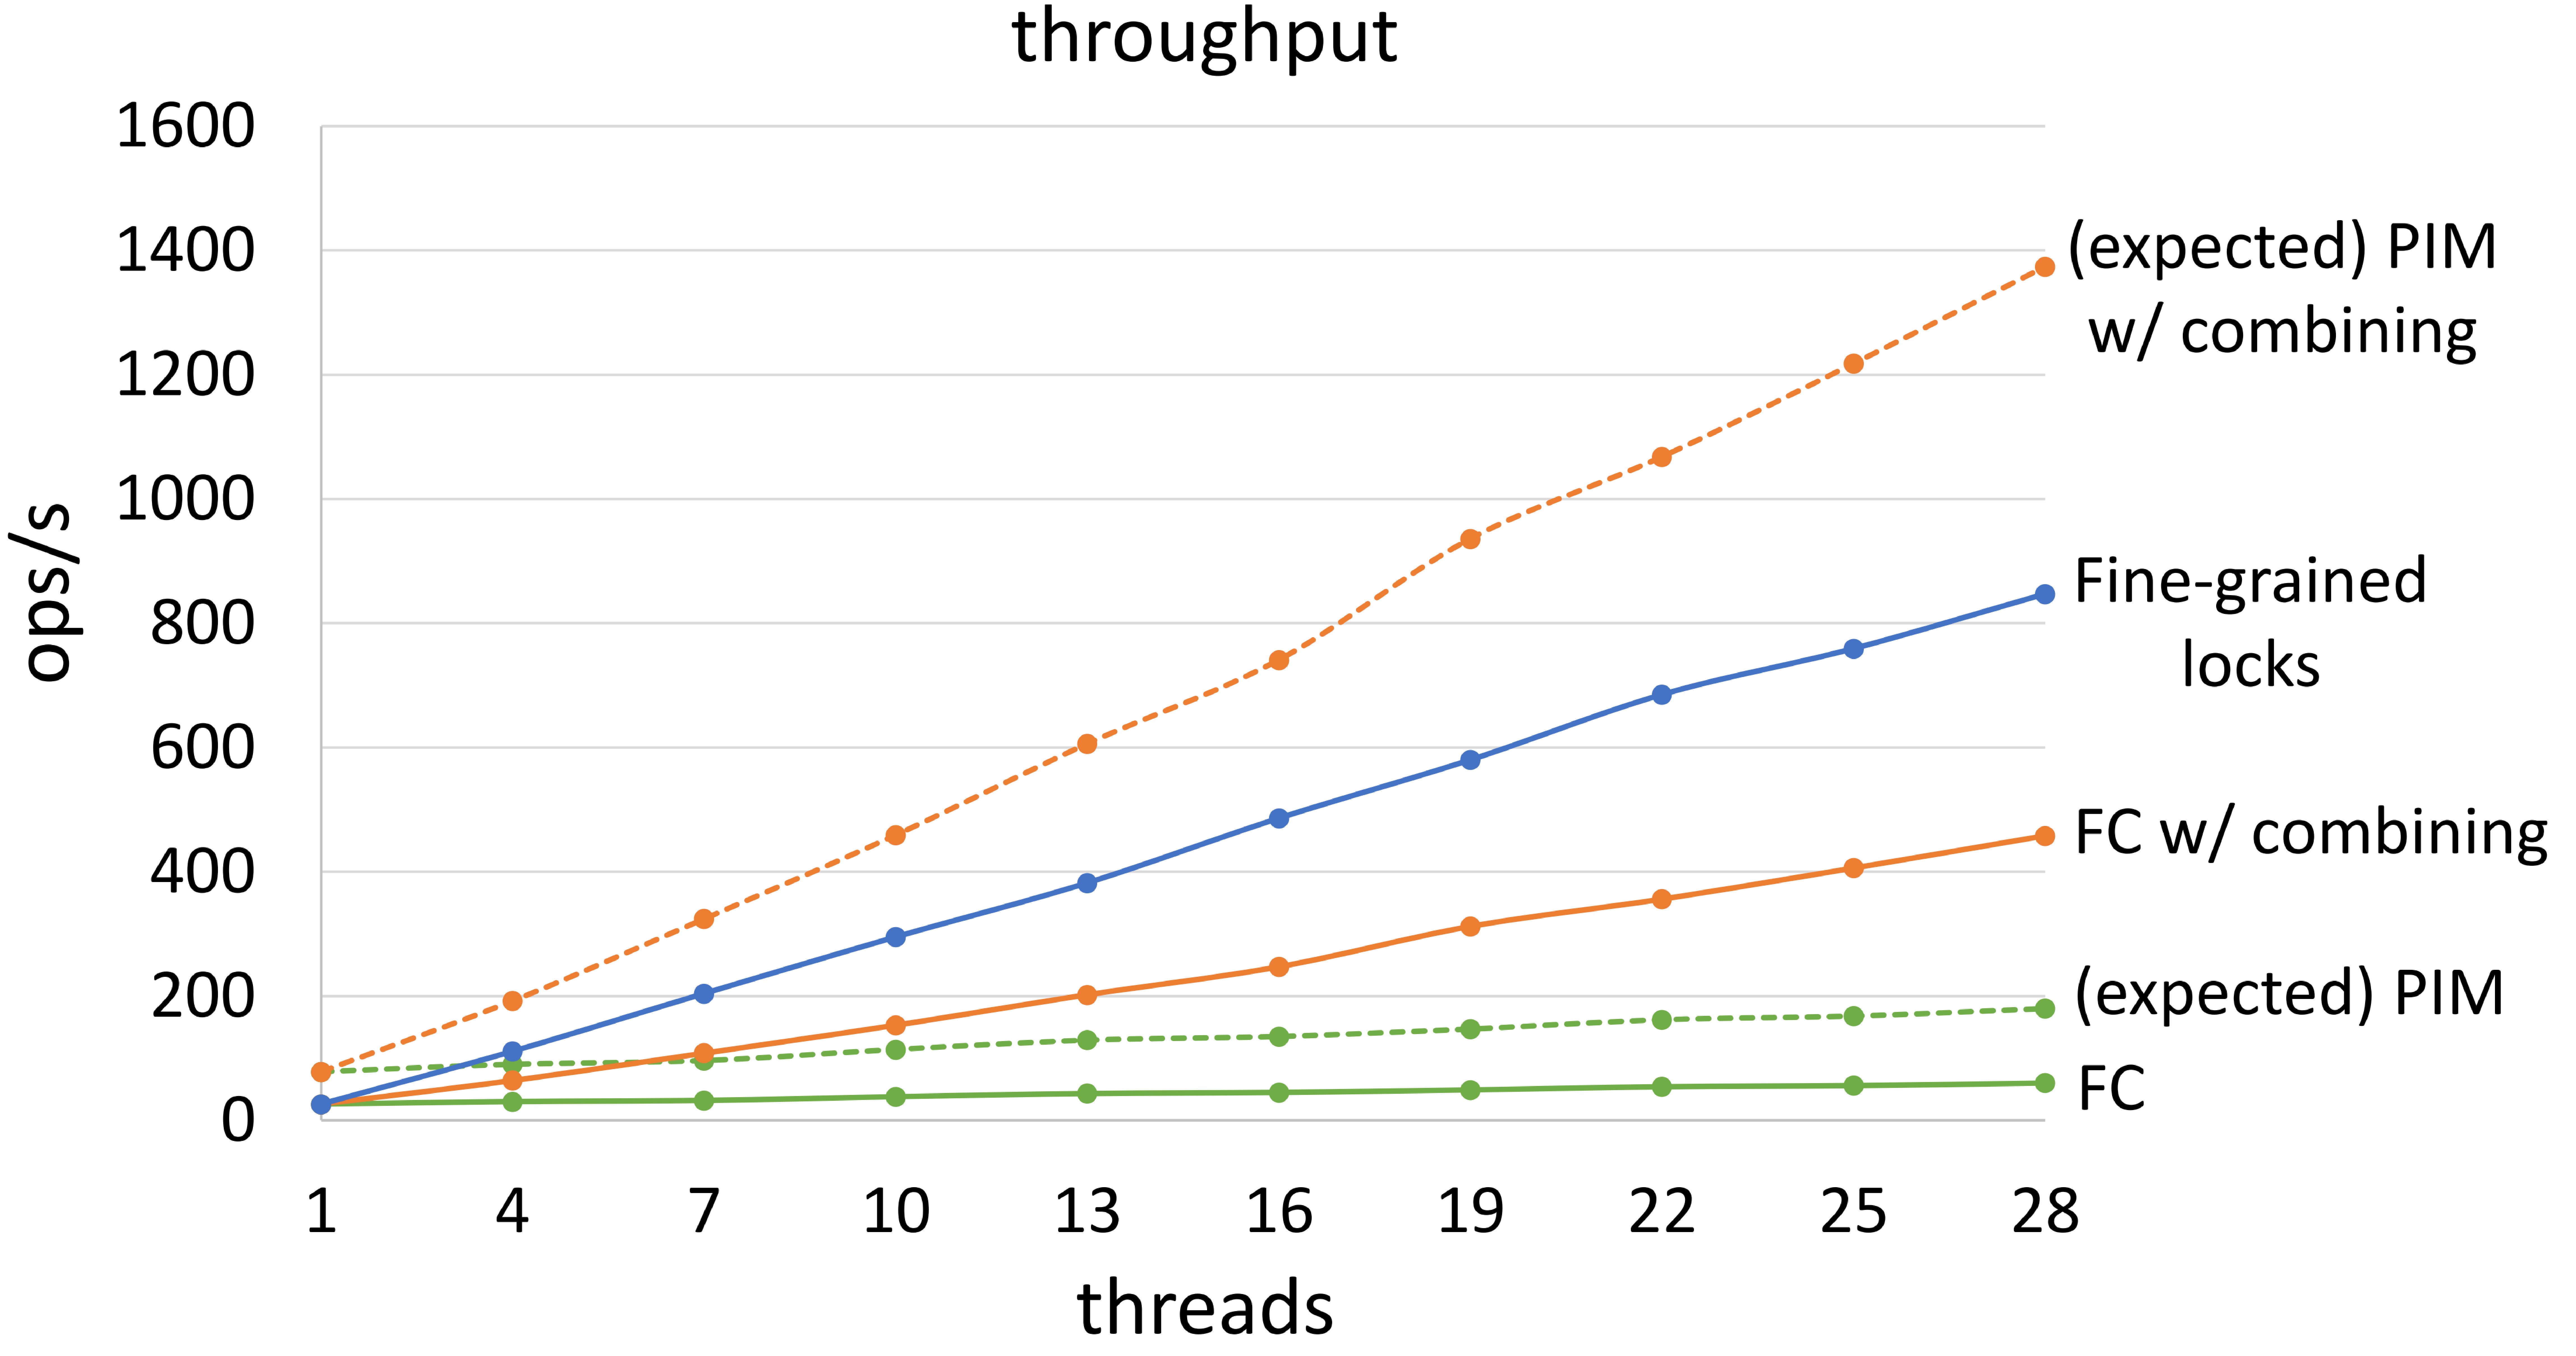
\includegraphics[width=.95\linewidth]{linkedlist_data.eps} 
    \caption{Experimental results of linked-lists. We evaluate the linked-list with fine-grained locks 
        and the flat-combining linked-list (FC) with and without the combining optimization.}
   \label{figure:linkedlist_data}
\end{figure}


\subsection{Skip-lists}
\label{section:skip_list}

%\subsubsection{Base algorithm}

Like the naive PIM-managed linked-list,
the naive PIM-managed skip-list keeps the skip-list in a single vault and
CPU cores send operation requests to the local PIM core that executes those operations.
As we will see, this skip-list is less efficient than some existing skip-list algorithms.

Unfortunately, the combining optimization \emph{cannot} be applied to skip-lists effectively.
The reason is that for any two distant nodes in the skip-list,
the paths threads must traverse to reach such nodes do \emph{not} have large overlapping sub-paths.

On the other hand, PIM memory usually consists of many vaults and PIM cores.
For instance, the first generation of Hybrid Memory Cube \cite{website:HMC} has up to 32 vaults.
Hence, a PIM-managed skip-list can achieve much better performance if
we can exploit the parallelism of multiple vaults.
Here we present our PIM-managed skip-list with a \textit{partitioning optimization}:
A skip-list is divided into partitions of disjoint ranges of keys,
stored in different vaults, so that a CPU sends its operation request to
the PIM core of the vault to which the key of the operation belongs.

Figure \ref{figure:skiplist_structure} illustrates the structure of a PIM-managed skip-list.
Each partition of a skip-list starts with a \textit{sentinel node}
which is a node with maximum height. 
For simplicity, assume that the max height $H_{max}$ is predefined.
A partition covers a key range between the key of its sentinel node and
the key of the sentinel node of the next partition.
CPUs also store a copy of each sentinel node in regular DRAM (see Figure~\ref{figure:model}) and 
this copy has an extra variable indicating the vault containing the sentinel node.
The number of nodes with max height is very small with high probability, 
so the sentinel nodes can likely be found in the CPU caches  
because CPUs access them frequently.

When a CPU performs an operation for a key on the skip-list,
it first compares the key with those of the sentinels, discovers which vault
the key belongs to, and then sends its operation request to that vault's PIM core.
After the PIM core retrieves the request, it executes the operation in the local vault 
and sends the result back to the CPU.


\begin{figure}[ht!]
%$\hrulefill$
%\\
%\\
\centering
\includegraphics[width=.8\linewidth]{skiplist_structure.eps}
%$\hrulefill$
\caption{A PIM-managed skip-list with three partitions}
\label{figure:skiplist_structure}
\end{figure}

We now discuss how we implement the PIM-managed skip-list
when the key of each operation is an integer generated uniformly at random
from range $[0, n]$ and the PIM memory has $k$ vaults available.
Initially we can create $k$ partitions starting with fake sentinel nodes
with keys $0$, $1/k$, $2/k$,..., $(n-1)/k$, respectively, 
and allocate each partition in a different vault. 
The sentinel nodes are never deleted.
If a new node to be added has the same key as a sentinel node,
we insert it immediately after the sentinel node.

We compare the performance of our PIM-managed skip-list with $k$ partitions 
to the performance of a flat-combining skip-list \cite{Hendler10}
and a lock-free skip-list \cite{Herlihy08}, 
accessed concurrently by $p$ CPUs.
We also apply the partitioning optimization to the flat-combining skip-list, 
so that $k$ combiners are in charge of $k$ partitions of the skip-list. 
To simplify the comparison, we assume that all skip-lists have the same
initial structure, i.e. skip-lists with partitions have extra sentinel nodes.
We execute an equal number of add() and remove() requests, so that the size of the 
skip-list does not change dramatically. 
The keys of requests are generated uniformly at random. 

The approximate throughput of each of these skip-lists is presented in Table \ref{tab:skiplist}, 
where $\beta$ is the average number of nodes an operation has to access 
in order to find the location of its key in a skip-list
($\beta = \Theta(\log N)$, where $N$ is the size of the skip-list).
In the lock-free skip-list, $p$ threads execute their own operations in parallel, 
so the throughput is roughly $p/(\beta\latcpu)$. 
Without the partitioning optimization, a combiner in the flat-combining skip-list and a PIM core 
in the PIM-managed skip-list both have to execute operations one by one sequentially, 
leading to throughput of roughly ${1 \over (\beta\latcpu)}$ and ${1 \over (\beta\latpim + \latmes)}$ respectively, 
where $\latmes$ is incurred by the PIM core sending a message with a result back to a CPU. 
After dividing these two skip-lists into $k$ partitions, we can achieve a speedup of $k$ for both of them, 
as $k$ PIM cores and $k$ combiners can serve requests in parallel now. 
Note that we have ignored certain costs in the lock-free skip-list and the two flat-combining skip-lists, 
such as the cost of a combiner's operations on the publication list in a flat-combining skip-list
and the cost of CAS operations in the lock-free skip-list, 
so their actual performance could be even worse than what we show in Table \ref{tab:skiplist}.  

\begin{table}[ht!]
\begin{center}
	\begin{tabular}{| >{\small}l | l |}
    %\begin{tabular}{| m{0.55\linewidth}  | c |}
    \hline
    \textbf{Algorithm} & \textbf{Throughput} \\ \hhline{|=|=|} 
    Lock-free skip-list & ${p \over \beta\latcpu}$ \\ \hline
    Flat-combining skip-list & ${1 \over \beta\latcpu}$ \\ \hline
    PIM-managed skip-list & ${1 \over (\beta\latpim + \latmes)}$ \\ \hline
    Flat-combining skip-list with $k$ partitions & ${k \over \beta\latcpu}$ \\ \hline
    PIM-managed skip-list with $k$ partitions & ${k \over (\beta\latpim + \latmes)}$ \\ \hline
    \end{tabular}
\end{center}
\caption{Throughput of skip-lists}
\label{tab:skiplist}
\end{table}

The results in Table \ref{tab:skiplist} imply that 
the PIM-managed skip-list with $k$ partitions is expected to outperform the second best skip-list, 
the lock-free skip-list, when $k > {(\beta\latpim + \latmes)p \over \beta\latcpu}$.
Given that $\latmes = \latcpu = r_1\latpim$ and $\beta = \Theta(\log N)$, $k > p/r_1$ should suffice.
It is also easy to see that the performance of the PIM-managed skip-list is  
${\beta r_1 \over \beta + r_1} \approx r_1$ times better than the flat-combining skip-list, 
when they have the same number of partitions. 

Our experimental evaluation reveals similar results, 
as presented in Figure \ref{figure:skiplist_data}.
We have implemented and run the flat-combining skip-list with different numbers of
partitions and compared them with the lock-free skip-list.
As the number of partitions increases, the performance of the flat-combining skip-list
improves, attesting to the effectiveness of the partitioning optimization.
Again, we believe the performance of the flat-combining skip-list is a good indicator
of the performance of our PIM-managed skip-list.
Therefore, according to the analytical results in Table \ref{tab:skiplist}, we can triple the throughput 
of a flat-combining skip-list to estimate the expected performance of a PIM-managed skip-list.
As Figure \ref{figure:skiplist_data} illustrates, when our PIM-managed skip-list has $8$ or $16$ 
partitions, it is expected to outperform the lock-free skip-list with up to 28 hardware threads.

\begin{figure}[ht!]
    \centering
    
\includegraphics[width=1.0\linewidth]{skiplist_data.eps} % second figure itself
    \caption{Experimental results of skip-lists. We evaluated the lock-free skip-list and 
    the flat-combining skip-list (FC) with different numbers (1, 4, 8, 16) of partitions.}
    \label{figure:skiplist_data}
\end{figure}


%\subsubsection{Rebalancing skip-list}
\subsubsection{Skip-list Rebalancing}
The PIM-managed skip-list performs well with a uniform distribution of requests.
However, if the distribution of requests is \emph{not} uniform, a static partitioning scheme 
will result in unbalanced partitions, with some PIM cores potentially being idle, while others having to 
serve a majority of the requests. To address this problem, we introduce a non-blocking protocol for 
migrating consecutive nodes from one vault to another. 

The protocol works as follows. 
A PIM core $p$ that manages a vault $v'$ can send a message to another PIM core $q$, managing vault 
$v$, to request some nodes to be moved from $v'$ to $v$. 
First, $p$ sends a message notifying $q$ of the start of the migration. 
Then $p$ sends messages to $q$ for adding those nodes into $v$ one by one in ascending order 
according to the keys of the nodes. 
After all the nodes have been migrated, $p$ sends notification messages to CPUs so that 
they can update their copies of sentinel nodes accordingly.
After $p$ receives acknowledgement messages from all CPUs, it notifies $q$ of the end of migration.
To keep the node migration protocol simple, we don't allow $q$ to move those nodes 
to another vault again until $p$ finishes its node migration. 

During the node migration, $p$ can still serve requests from CPUs.
Assume that a request with key $k_1$ is sent to $p$ when $p$ is migrating nodes 
in a key range containing $k_1$.  
If $p$ is about to migrate a node with key $k_2$ at the moment and $k_1 \ge k_2$, 
$p$ serves the request itself. 
Otherwise, $p$ must have migrated all nodes in the subset containing key $k_1$, and therefore $p$ 
forwards the request to $q$ which will serve the request and respond directly to the requesting CPU. 

This skip-list is correct, because a request will eventually reach the vault that 
currently contains nodes in the key range that the request belongs to. 
If a request arrives to $p$ which no longer holds the partition the request belongs to, 
$p$ simply replies with a rejection to the CPU and the CPU will resend its request to 
the correct PIM core, 
because it has already updated its sentinels and knows which PIM core it should contact now. 

Using this node migration protocol, the PIM-managed FIFO queue can support two rebalancing schemes:
1) If a partition has too many nodes, the local PIM core can move nodes in a key range to a vault 
that has fewer nodes;
2) If two consecutive partitions are both small, 
we can merge then by moving one to the vault containing the other. 

In practice, we expect that rebalancing will not happen very frequently, so its overhead can be 
ameliorated by the improved efficiency resulting from the rebalanced partitions. 

